% Copyright 2004 by Till Tantau <tantau@users.sourceforge.net>.
%
% In principle, this file can be redistributed and/or modified under
% the terms of the GNU Public License, version 2.
%
% However, this file is supposed to be a template to be modified
% for your own needs. For this reason, if you use this file as a
% template and not specifically distribute it as part of a another
% package/program, I grant the extra permission to freely copy and
% modify this file as you see fit and even to delete this copyright
% notice. 

\documentclass{beamer}

\newcommand{\bO}{\mathcal{O}}

% There are many different themes available for Beamer. A comprehensive
% list with examples is given here:
% http://deic.uab.es/~iblanes/beamer_gallery/index_by_theme.html
% You can uncomment the themes below if you would like to use a different
% one:
%\usetheme{AnnArbor}
%\usetheme{Antibes}
%\usetheme{Bergen}
%\usetheme{Berkeley}
%\usetheme{Berlin}
%\usetheme{Boadilla}
%\usetheme{boxes}
%\usetheme{CambridgeUS}
%\usetheme{Copenhagen}
%\usetheme{Darmstadt}
%\usetheme{default}
%\usetheme{Frankfurt}
%\usetheme{Goettingen}
%\usetheme{Hannover}
%\usetheme{Ilmenau}
%\usetheme{JuanLesPins}
%\usetheme{Luebeck}
\usetheme{Madrid}
%\usetheme{Malmoe}
%\usetheme{Marburg}
%\usetheme{Montpellier}
%\usetheme{PaloAlto}
%\usetheme{Pittsburgh}
%\usetheme{Rochester}
%\usetheme{Singapore}
%\usetheme{Szeged}
%\usetheme{Warsaw}

\title{Computational Methods for Principle Component Analysis}

% A subtitle is optional and this may be deleted
% \subtitle{Optional Subtitle}

\author{David Zhang}
% - Give the names in the same order as the appear in the paper.
% - Use the \inst{?} command only if the authors have different
%   affiliation.

\date{20 April 2018}
% - Either use conference name or its abbreviation.
% - Not really informative to the audience, more for people (including
%   yourself) who are reading the slides online

% \subject{Theoretical Computer Science}
% This is only inserted into the PDF information catalog. Can be left
% out. 

% If you have a file called "university-logo-filename.xxx", where xxx
% is a graphic format that can be processed by latex or pdflatex,
% resp., then you can add a logo as follows:

% \pgfdeclareimage[height=0.5cm]{university-logo}{university-logo-filename}
% \logo{\pgfuseimage{university-logo}}

% Let's get started
\begin{document}

\begin{frame}
  \titlepage
\end{frame}

% Section and subsections will appear in the presentation overview
% and table of contents.
\section{First Main Section}

\subsection{First Subsection}

\begin{frame}{Recap of Principle Component Analysis (PCA)}
\begin{itemize}
\item PC scores capture ancestral history well
\item PCA by singular value decomposition (SVD)
    \[
        \underset{p \times n}{X} = \underset{p \times n}{U} \; \underset{n \times n}{D} \; \underset{n \times n}{V^T}
    \]
    \begin{itemize}
        \item $p$: \# Features (SNPs)
        \item $n$: \# Individuals
        \item $U$: PC loadings (direction vectors)
        \item $D$: Diagonal matrix of PC standard deviations (descending)
        \item $V$: PC scores (what we are the most interested in)
    \end{itemize}
\item Can also use eigen decomposition
    \[
        X^T X = VD^2V^T, \quad X X^T = U D^2 U^T
    \]
\item When applied to all the study samples,
    the PC scores capture the population stratification (PS) well
\end{itemize}
\end{frame}

\begin{frame}{Predicting PC scores}
\begin{itemize}
\item Instead of applying PCA to all the study samples
    \begin{itemize}
    \item apply PCA to reference samples
    \item use reference PC scores to predict each study sample's PC scores
    \end{itemize}
\item Methods
    \begin{itemize}
    \item Simple Projection (SP)
    \item Adjusted Projection (AP)
        \cite{dey2016asymptotic}
    \item Augment, Decompose, Procrustes (ADP) 
        \cite{wang2015improved}
    \item Online ADP (OADP)
        \cite{brand2002incremental}
    \end{itemize}
\end{itemize}
\end{frame}

\begin{frame}{Simple Projection (SP)}
\begin{itemize}
\item Algorithm
    \begin{enumerate}
    \item SVD on reference samples
        \[
            X_{ref} = U_{ref} D_{ref} V_{ref}^T
        \]
    \item Project the new study sample to the reference PC loadings
        \[
           v_{new} = U_{ref}^T \; x_{new}
        \]
    \end{enumerate}
\item Pro: Fast and simple to implement $\bO[mkp]$
    \begin{itemize}
    \item $m$: \# study samples
    \item $k$: \# PCs needed
    \item $p$: \# SNPs 
    \end{itemize}
\item Con: PC scores shrink toward zero when $p >> n$
\end{itemize}
\end{frame}

\begin{frame}{Adjusted Projection (AP)}
\begin{itemize}
\item Algorithm
    \begin{enumerate}
    \item SVD on reference samples
        \[
            X_{ref} = U_{ref} D_{ref} V_{ref}^T
        \]
    \item Project the new study sample to the reference PC loadings
        \[
           v_{new} = U_{ref}^T \; x_{new}
        \]
    \item \textcolor{red}{Estimate the magnitude and angle of the shrinkage by using $D_{ref}^2$}
    \item \textcolor{red}{Adjust $v_{new}$ for this shrinkage}
    \end{enumerate}
\item Computational complexity is the same as SP $\bO[mkp]$
\item Empirical runtime slightly higher than SP
\item Software: HDPCA (R package)
\end{itemize}
\end{frame}

\begin{frame}{Augment, Decompose, Procrustes (ADP)}
\begin{enumerate}
\item Calculate the reference covariance matrix $X_{ref}^T X_{ref}$
\item Eigendecomposition on the reference covariance matrix:
\[
    X_{ref}^T X_{ref} = V_{ref} D_{ref}^2 V_{ref}^T
\]
\item Augment the reference samples by appending the new study sample: $X_{aug} = (X_{ref}, x_{new})$
\item Find the augmented covariance matrix $X_{aug}^T X_{aug}$
\item Eigendecomposition on the augmented covariance matrix
\[
    X_{aug}^T X_{aug} = V_{aug} D_{aug}^2 V_{aug}^T
\]
\item Divide the augmented PC scores into the reference part and the new part: $V_{aug}^T = (V_{aug, ref}^T, v_{aug, new}^T)$
\item Find a linear transformation $f(X) = \rho XA + b$ that minimizes the difference between $f(V_{aug,ref})$ and $V_{ref}$ (Procrustes analysis)
\item Apply the same transformation to $v_{aug,new}$ to get $f(v_{aug,new})$
\end{enumerate}
\end{frame}

\begin{frame}{Augment, Decompose, Procrustes (ADP)}
    \begin{itemize}
    \item Pro: Very accurate (The golden standard)
    \item Con: Very slow when reference size is large $\bO[m(np+n^3)]$
        \begin{itemize}
        \item $m$: \# study samples
        \item $n$: \# reference samples
        \item $p$: \# features
        \end{itemize}
    \item Software: TRACE (written in C++) 
    \end{itemize}
\end{frame}

\begin{frame}{Online Augment, Decompose, Procrustes (OADP)}
\begin{itemize}
\item Algorithm
    \begin{enumerate}
    \item \textcolor{red}{SVD on the reference samples}
        \[
            X_{ref} = U_{ref} D_{ref} V_{ref}^T
        \]
    \item \textcolor{red}{Update $V_{ref}$ into $V_{aug}$ by using $U_{ref}$, $D_{ref}$, and $x_{new}$}
    \item Divide the augmented PC scores
        into the reference part and the new part:
        $V_{aug}^T = (V_{aug, ref}^T, v_{aug, new}^T)$
    \item Find a linear transformation
        $f(X) = \rho XA + b$ 
        that minimizes the difference between
        $f(V_{aug,ref})$ and $V_{ref}$
        (Procrustes analysis)
    \item Apply the same transformation to $v_{aug,new}$
        to get $f(v_{aug,new})$
    \end{enumerate}
\item Speed up ADP by avoiding repetitive calculations
    ($\bO[mk(p+kn)])$
    \begin{itemize}
    \item $m$: \# study samples
    \item $k$: \# PCs needed
    \item $p$: \# features
    \end{itemize}
\item PC scores are almost identical to ADP's
\end{itemize}
\end{frame}

\begin{frame}{Application to Real Data}
\begin{itemize}
    \item Reference samples: 1000 Genomes Project
        \begin{itemize}
        \item 2492 individuals from 26 populations in Africa, America, East Asia, South Asia, and Europe
        \item 84M SNPs
        \item 627K SNPS left after intersecting with the Human Genome Diversity Project (HGDP)
        \end{itemize}
    \item Study samples: UK Biobank
        \begin{itemize}
        \item 488K individuals studied at 23 centers in UK
        \item 148K SNPs
        \end{itemize}
    \item \# Shared SNPs between reference and study samples: 18k
\end{itemize}
\end{frame}

\begin{frame}{1000 Genomes and UK Biobank (1000 Global Individuals)}
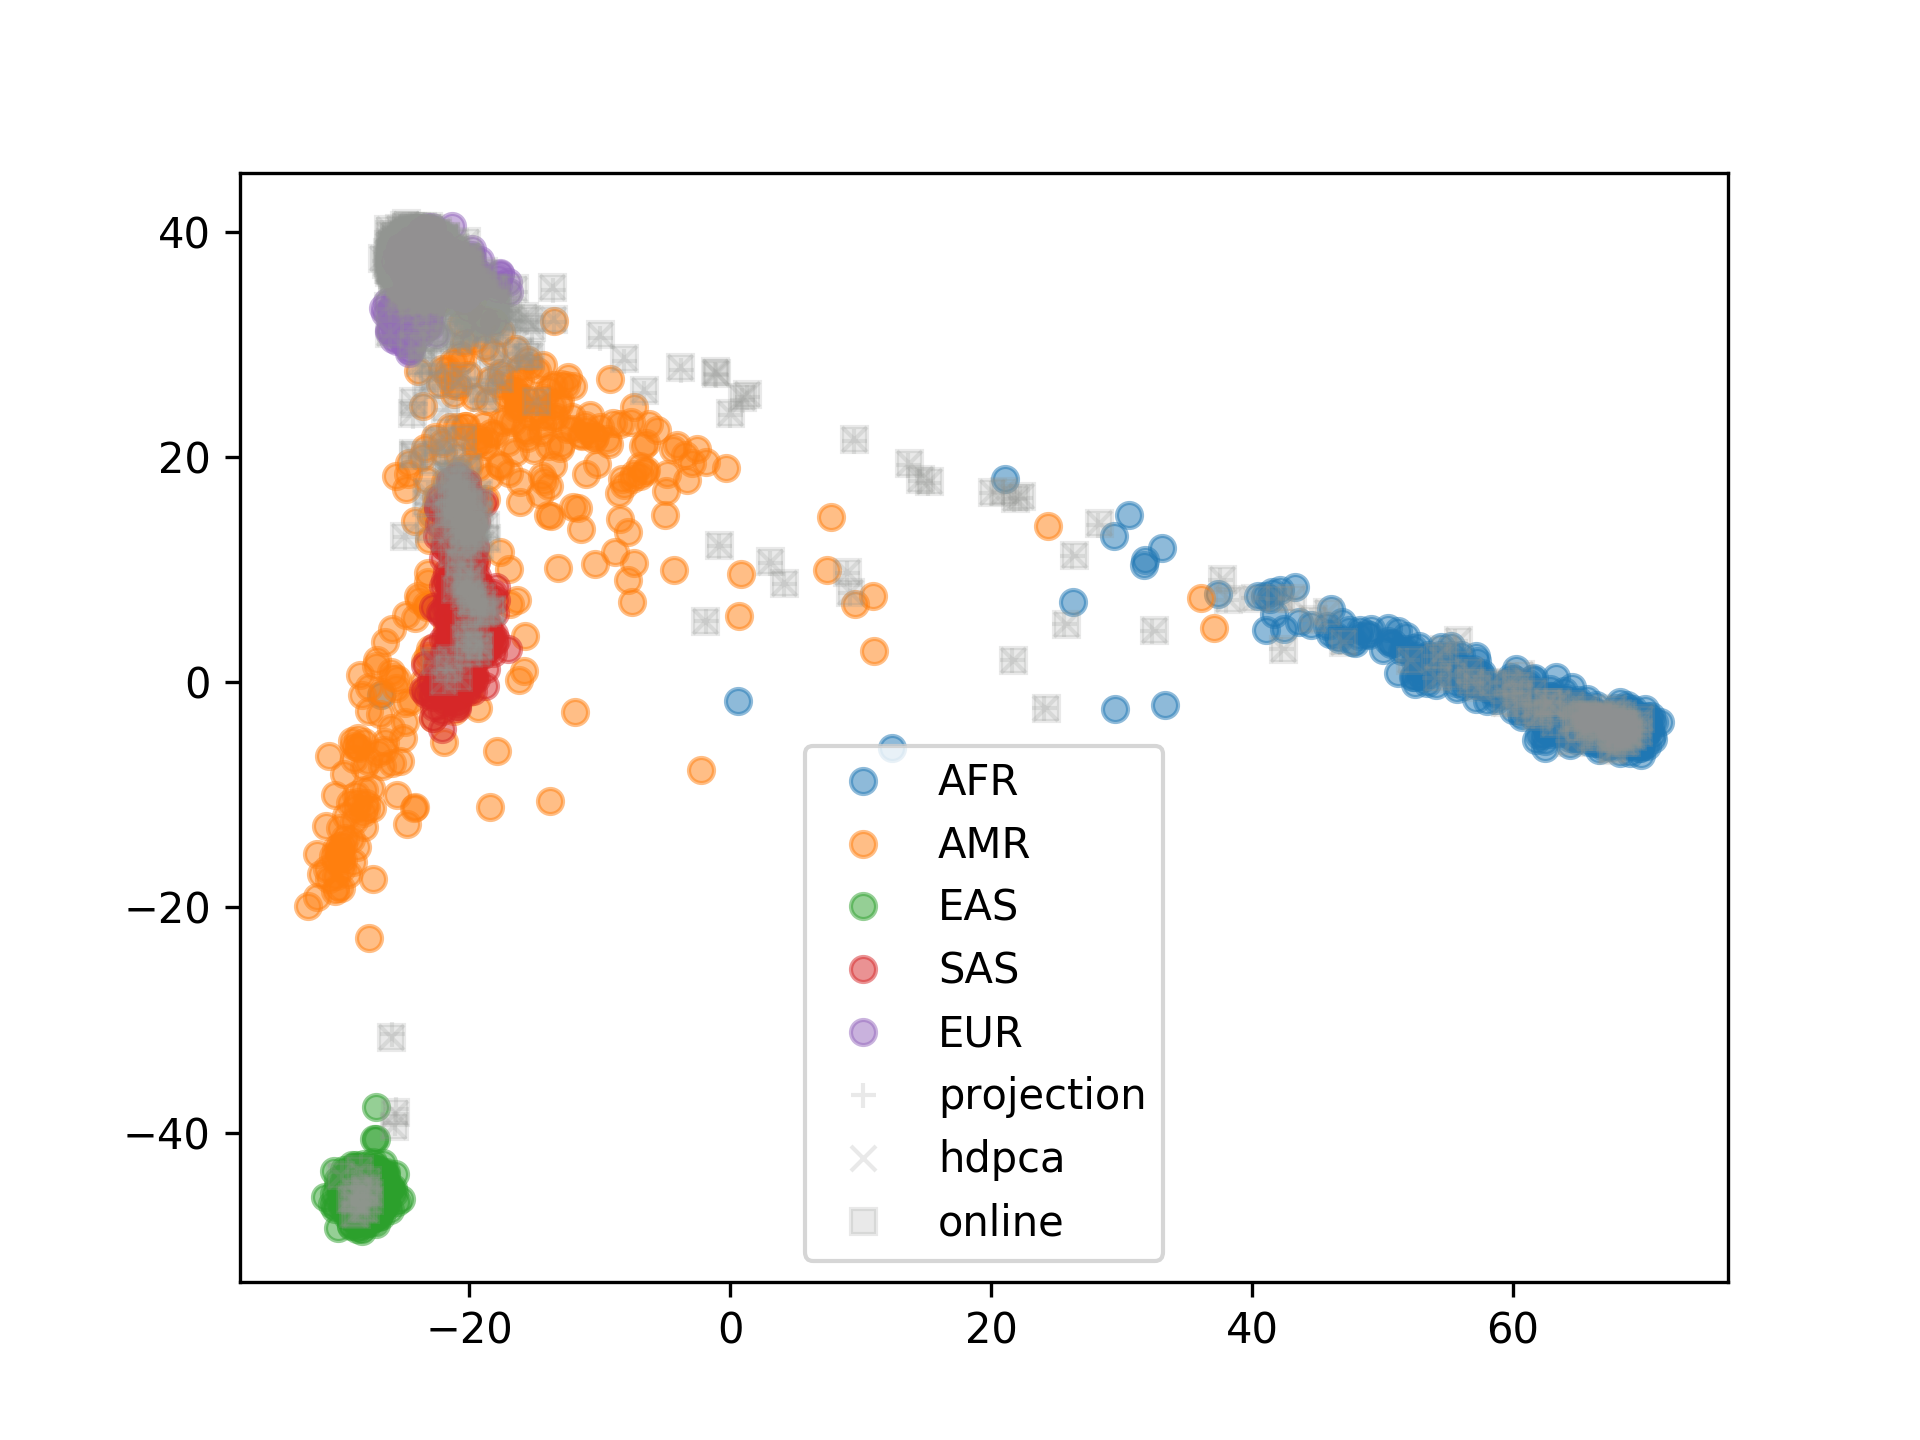
\includegraphics[height=0.9\textheight]{pcs_save.png}
\end{frame}

\begin{frame}{1000 Genomes and UK Biobank (Global)}
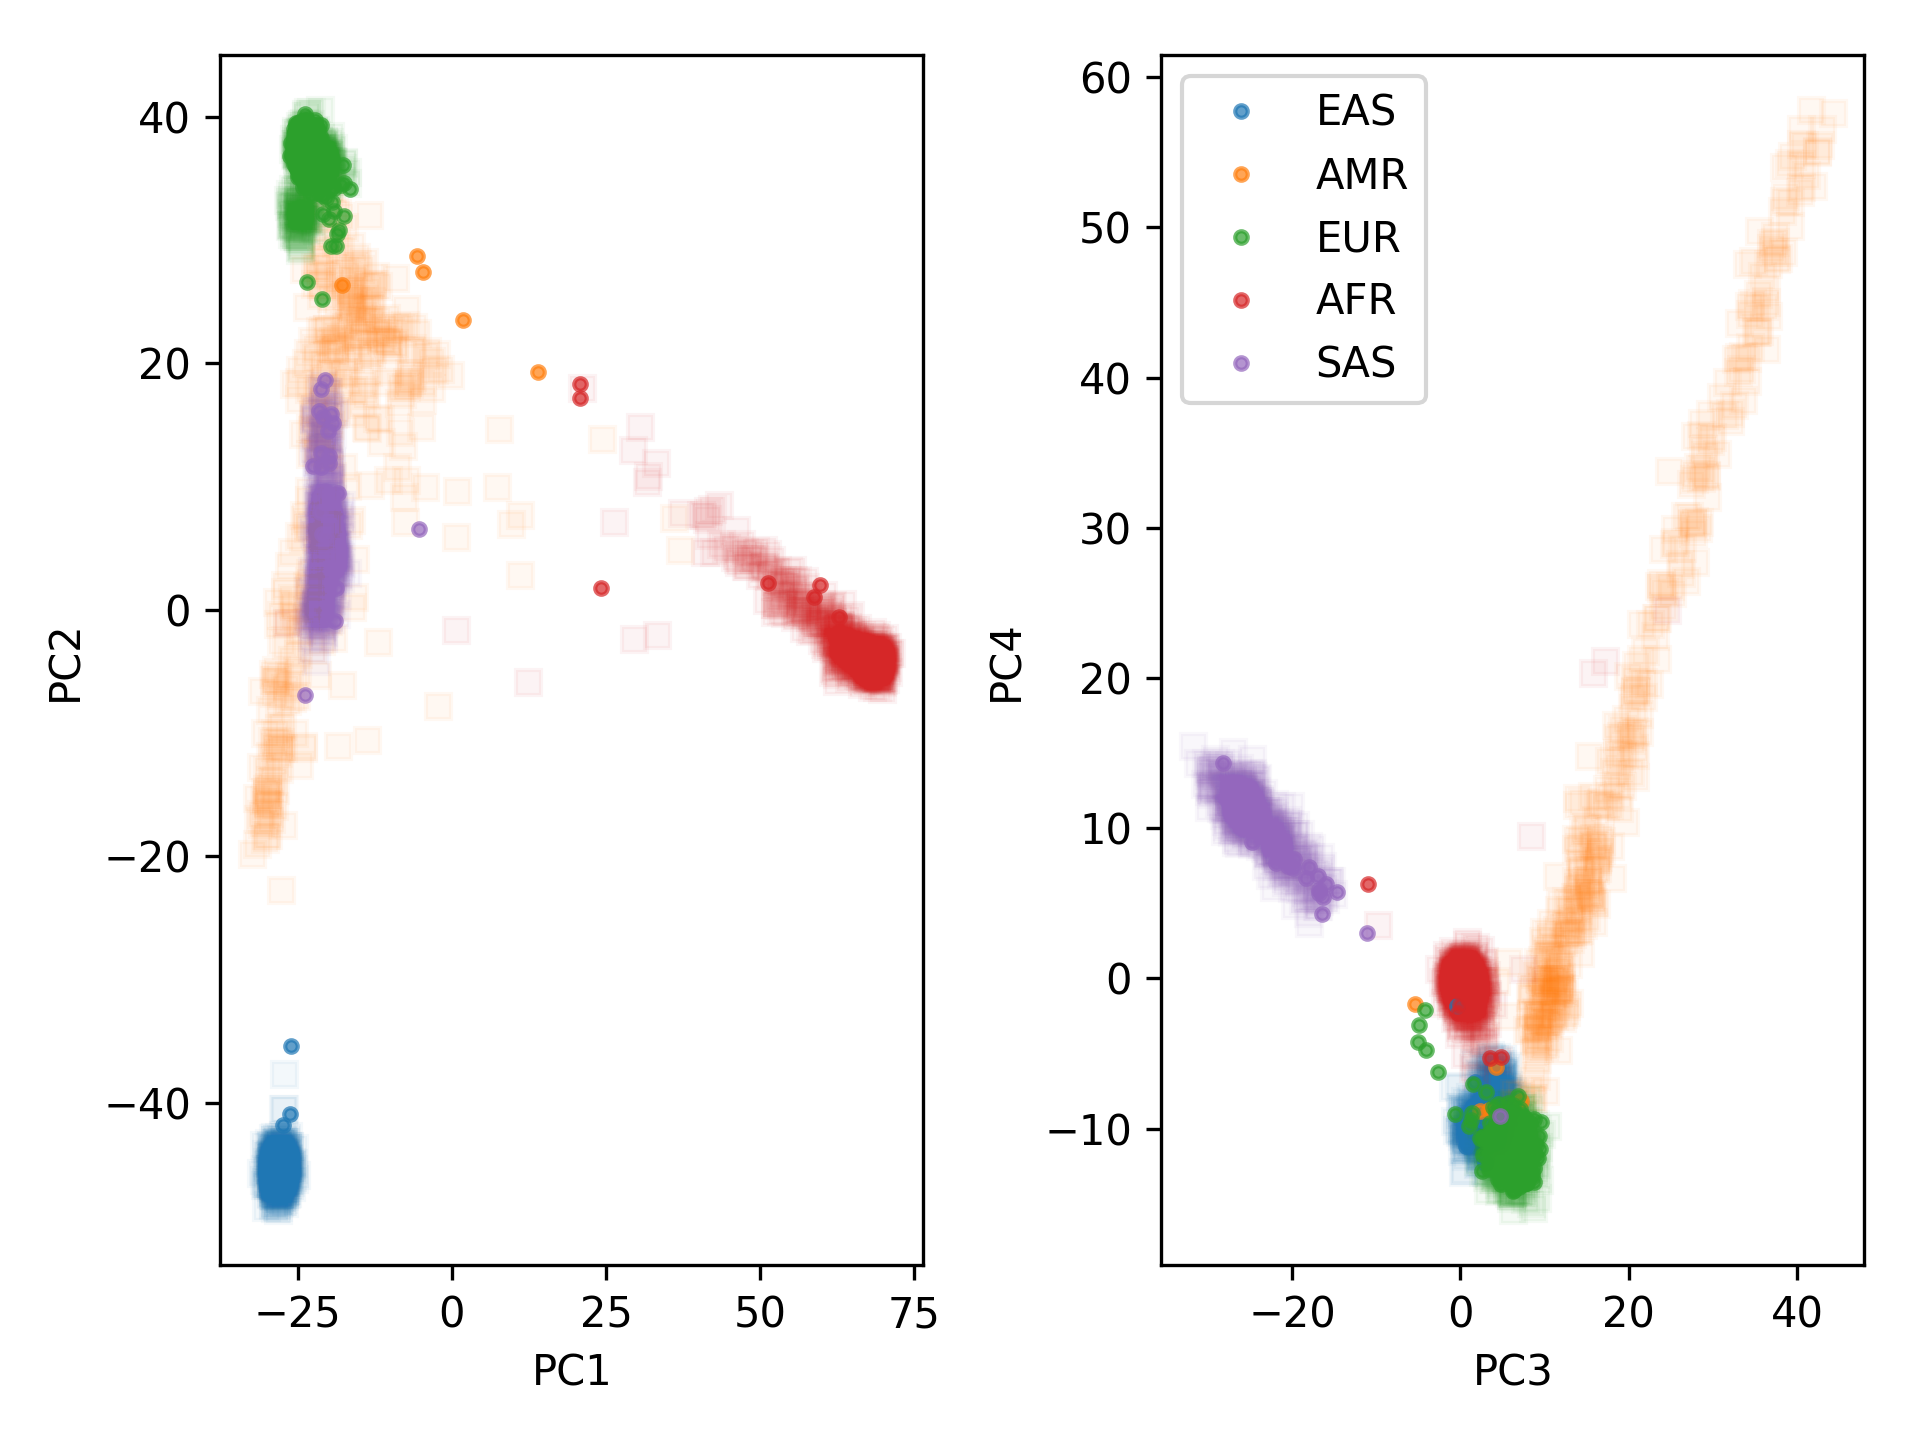
\includegraphics[height=0.9\textheight]{ukb_snps_kgn_1k.png}
\end{frame}

\begin{frame}{1000 Genomes and UK Biobank (Predicted Europeans)}
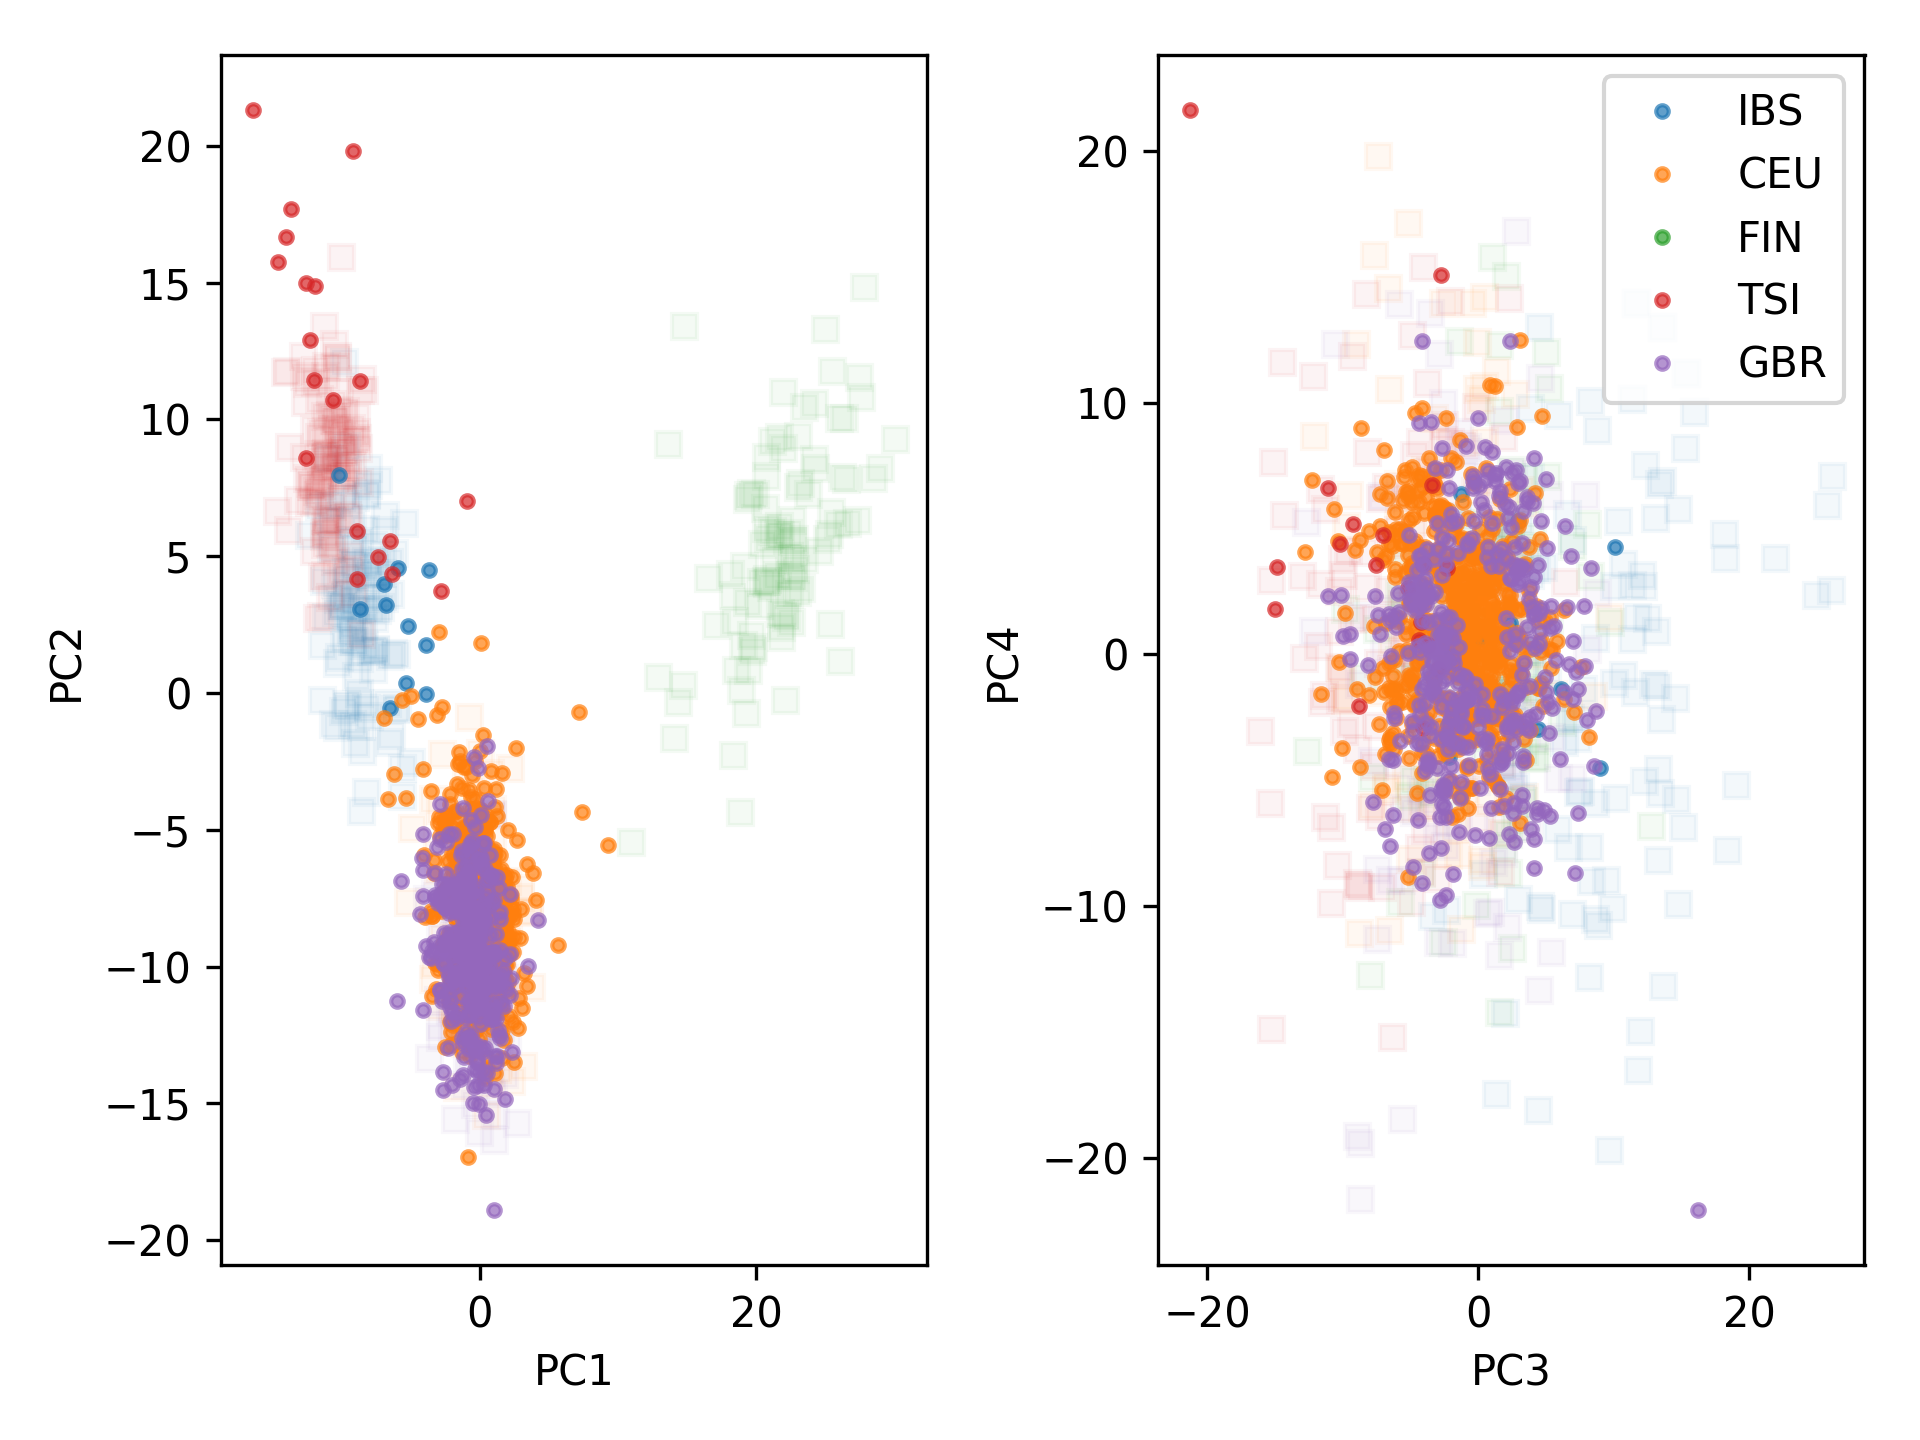
\includegraphics[height=0.9\textheight]{ukb_snps_kgn_1k_eur.png}
\end{frame}


\begin{frame}{1000 Genomes and UK Biobank (488K Global Individuals)}
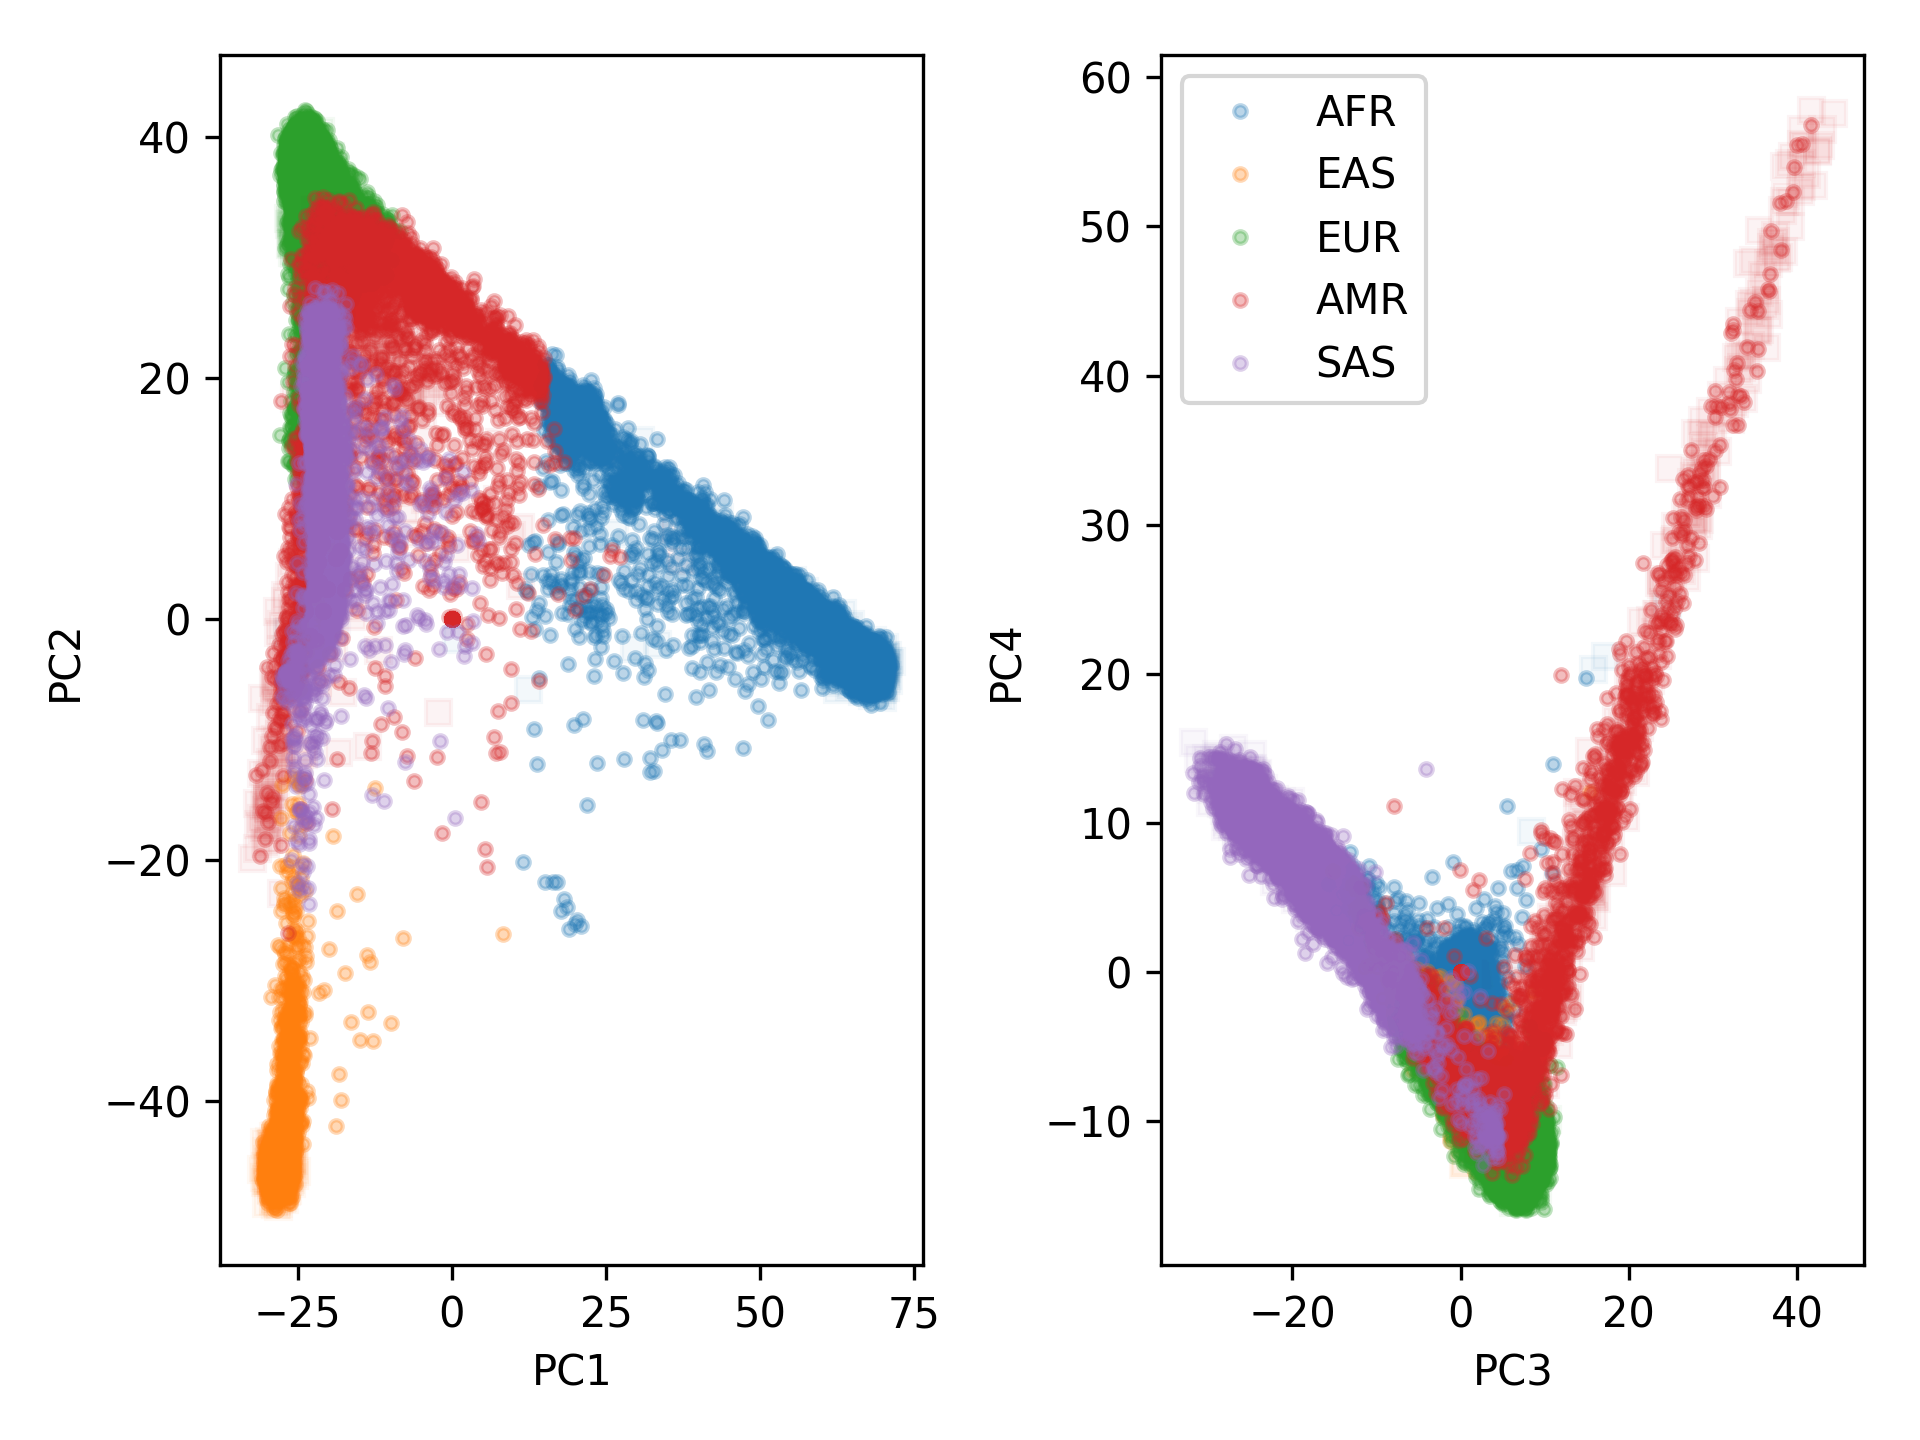
\includegraphics[height=0.9\textheight]{ukb_snps_kgn.png}
\end{frame}


\begin{frame}{Comparison of Efficiency}
\begin{table} 
  \centering
  \begin{tabular}{|l|l|l|l|}
    \hline
    & Reference & Study & UK Biobank \\
    Method & Complexity & Complexity & Study Runtime \\ 
    \hline
    SP & $\bO[n^2p]$ & $\bO[mkp]$ & 22 seconds \\
    \hline
    AP & $\bO[n^2p]$ &  $\bO[mkp]$ & 2.4 hours \\
    \hline
    ADP & $\bO[n^2 p]$ & $\bO[mn(p + n^2)]$ & 76 days* \\
    \hline
    OADP & $\bO[n^2 p]$ & $\bO[mk(p + k n)]$ & 4.8 hours \\
    \hline
  \end{tabular}
\end{table}

*Estimated by using the record that 1000 study samples took 3.75 hours.
\end{frame}


\begin{frame}{References}
    \bibliographystyle{apalike}
    \bibliography{main}
\end{frame}

\end{document}


